Das Backend soll wie in Kapitel 2.3 beschrieben die Datenquelle f�r die
verschiedenen Clients sein. Umgesetzt werden soll dies �ber einen RESTful
Service. Es wird das Framework "`Spring"' eingesetzt. Dies erlaubt eine einfache
Erstellung von Web-Services und unterst�tzt den Programmierer mit Werkzeugen wie
Hibernate, die die Verwaltung der Datenbank stark vereinfacht und �nderungen an
der Modellierung direkt in der Datenbank umsetzt.
\subsection{Anforderungen}
Wie oben genannt soll das Backend als RESTful-Service gestaltet werden. D
\subsection{Implementierung}

	\subsubsection{Datenbank}
	
	 \begin{figure}[H]
		\begin{minipage}{\linewidth}
		 	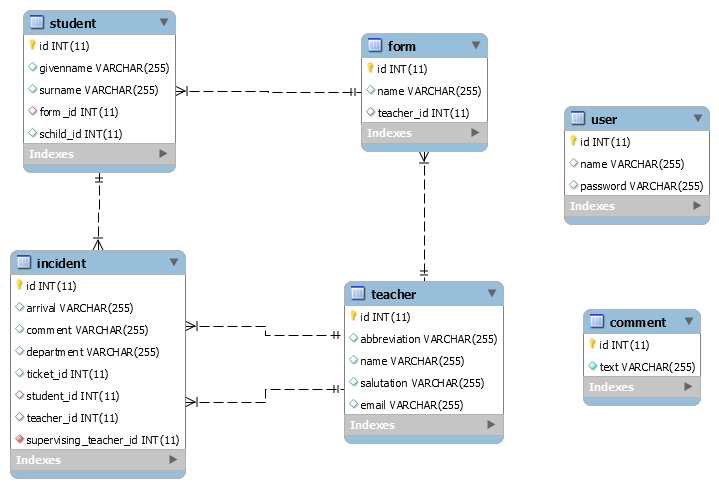
\includegraphics[width=0.9\linewidth]{grafx/ER_Model}
 			\caption[ER-Modell der Datenbank]{ER-Modell der Datenbank}
  			\label{fig:er_model}
		\end{minipage}
	\end{figure}

\subsection{Tests }


	\subsubsection{In Memory DB ?}


\subsection{Generischer Controller ??}
 